\section{Results}
\label{sec:results}

\subsection{H-E3: Per-Sample Hessian Trace Discriminates Minority Group Membership}

\textbf{Main result:} 4/5 seeds satisfy all three gate criteria simultaneously. Per-sample last-fc Hessian trace achieves AUROC$\geq$0.85 for minority membership prediction at $t^*$, with the signal being ERM-induced (AUROC$(t{=}0)<0.70$ in all seeds), and developing monotonically in 4/5 seeds (Spearman $\rho\geq$0.8).

\subsubsection*{Per-Seed AUROC Results}

\begin{table}[h]
\centering
\caption{Per-seed AUROC results for H-E3 existence gate.}
\label{tab:auroc}
\begin{tabular}{@{}lrrrrr@{}}
\toprule
Seed & AUROC$(t{=}0)$ & AUROC$(t^*)$ & $t^*$ & Spearman $\rho$ & Pass \\
\midrule
1 & 0.538 & 0.850 & 20 & 0.70 & $\times$ \\
2 & 0.609 & 0.885 & 50 & 0.943 & $\checkmark$ \\
3 & 0.558 & 0.897 & 50 & 0.943 & $\checkmark$ \\
4 & 0.579 & 0.903 & 20 & 0.900 & $\checkmark$ \\
5 & 0.609 & 0.890 & 5  & 1.000 & $\checkmark$ \\
\bottomrule
\end{tabular}
\end{table}

\textbf{Gate result: PASS (4/5 seeds).} Seed 1 fails due to a non-monotone AUROC trajectory (Spearman $\rho{=}0.70$, threshold 0.80) caused by a dip at $t{=}5$ --- both AUROC$(t{=}0)<0.70$ and AUROC$(t^*)\geq 0.85$ are satisfied.

\textbf{Epoch-0 control:} All 5 seeds show AUROC$(t{=}0)\in[0.538, 0.609]$ (mean 0.577) --- well below the 0.70 control threshold. The pretrained ImageNet backbone alone does not discriminate minority from majority training samples on Waterbirds. The trace asymmetry is created by ERM training.

Figure~\ref{fig:gate_metrics} shows AUROC$(t{=}0)$ and AUROC$(t^*)$ per seed with gate thresholds. Figure~\ref{fig:auroc_trajectory} shows the full AUROC trajectory across all 6 checkpoints.

\subsubsection*{Trace Ratio $R(t)$}

The trace ratio $R(t) = \overline{\text{trace}}_{\text{min}} / \overline{\text{trace}}_{\text{maj}}$ rises from near-unity at initialization to peak values of 4.09--8.89:

\begin{table}[h]
\centering
\caption{Trace ratio $R(t)$ at initialization and optimal checkpoint $t^*$.}
\label{tab:ratio}
\begin{tabular}{@{}lrrr@{}}
\toprule
Seed & $R(t{=}0)$ & $R(t^*)$ & $t^*$ \\
\midrule
1 & 1.05 & 4.37 & 20 \\
2 & 1.12 & 5.55 & 50 \\
3 & 1.06 & 7.21 & 50 \\
4 & 1.08 & 4.09 & 20 \\
5 & 1.12 & 8.89 & 5  \\
\bottomrule
\end{tabular}
\end{table}

All seeds show $R(t^*)\gg 1$ --- minority Hessian traces are systematically higher than majority at the peak checkpoint. Figure~\ref{fig:R_trajectory} shows the $R(t)$ trajectory for all seeds.

\subsubsection*{Estimator Stability}

\begin{table}[h]
\centering
\caption{Hutchinson coefficient of variation (CV) across $K{=}50$ probes.}
\label{tab:cv}
\begin{tabular}{@{}lr@{}}
\toprule
Seed & CV \\
\midrule
1 & 0.0233 \\
2 & 0.0132 \\
3 & 0.0232 \\
4 & 0.0283 \\
5 & 0.0108 \\
\bottomrule
\end{tabular}
\end{table}

All CVs $<$ 3\% (max 0.0283). $K{=}50$ Rademacher probes provide reliable per-sample trace estimates for the last-fc layer of ResNet-50. Figure~\ref{fig:trace_dist} shows the per-sample trace distributions at $t^*$.

\subsection{H-M1: Confidence-Differential Mechanism Is Absent at $t^*$}

\textbf{Main result:} The pre-registered mechanism gate fails in all 5 seeds. Minority training confidence at $t^*$ is 0.9678--0.9999 --- fully saturated, not boundary-straddling. The confidence-differential mechanism is inactive.

\begin{table}[h]
\centering
\caption{Per-seed training confidence at $t^*$ for H-M1 mechanism gate.}
\label{tab:confidence}
\begin{tabular}{@{}lrrrr@{}}
\toprule
Seed & $t^*$ & $p_{\text{min}}(t^*)$ & $p_{\text{maj}}(t^*)$ & Boundary $[0.3,0.7]$? \\
\midrule
1 & 20 & 0.9956 & 0.9994 & $\times$ \\
2 & 50 & 0.9999 & 0.9999 & $\times$ \\
3 & 50 & 0.9998 & 0.9999 & $\times$ \\
4 & 20 & 0.9964 & 0.9992 & $\times$ \\
5 & 5  & 0.9678 & 0.9925 & $\times$ \\
\bottomrule
\end{tabular}
\end{table}

\textbf{Gate result: FAIL (0/5 seeds).} No seed shows minority confidence in the predicted boundary condition range $[0.3, 0.7]$ at $t^*$. Mean $p_{\text{min}}(t^*)=0.9919$, mean $p_{\text{maj}}(t^*)=0.9982$.

\textbf{Transient early-epoch differential exists:} At epoch 1, a minority-majority confidence gap is visible (seed 1: $p_{\text{min}}=0.827$ vs $p_{\text{maj}}=0.972$). This is consistent with \cite{labonte2026phase}'s Phase I prediction --- ERM learns the spurious feature first, temporarily lagging minority confidence. However, this differential disappears before $t^*$ in all seeds.

\begin{figure}[h]
\centering
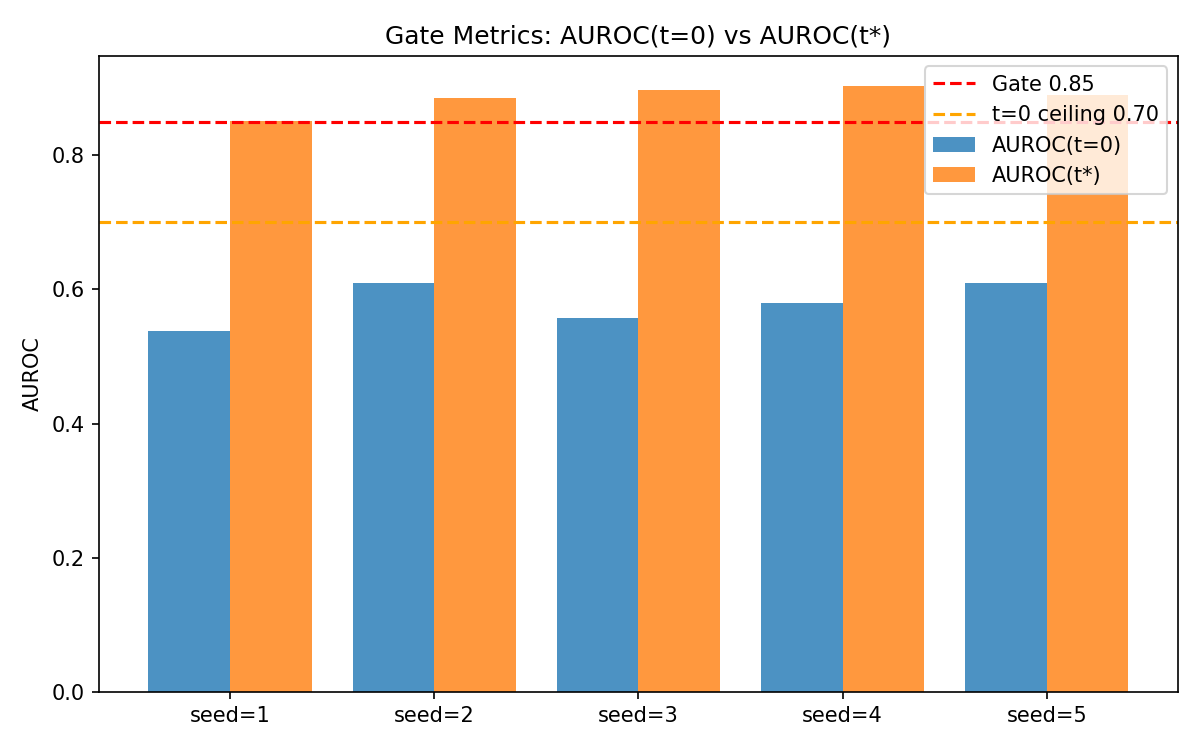
\includegraphics[width=0.8\columnwidth]{figures/fig1_gate_metrics.png}
\caption{AUROC at epoch 0 and at $t^*$ per seed, with gate thresholds (dashed lines). 4/5 seeds pass the H-E3 gate (AUROC$(t^*)\geq$0.85 and AUROC$(t{=}0)<$0.70).}
\label{fig:gate_metrics}
\end{figure}

\begin{figure}[h]
\centering
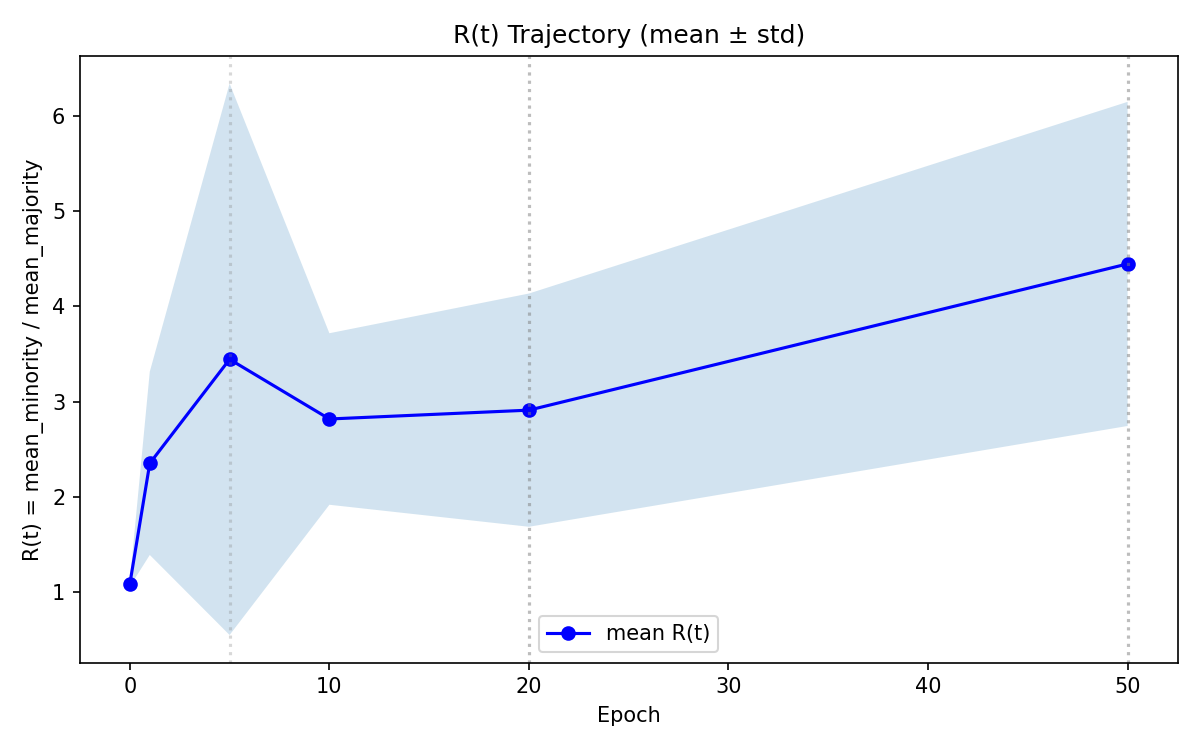
\includegraphics[width=0.8\columnwidth]{figures/fig2_R_trajectory.png}
\caption{Trace ratio $R(t)$ across training epochs for all 5 seeds. All seeds show $R(t^*)\gg 1$ indicating systematic minority trace elevation.}
\label{fig:R_trajectory}
\end{figure}

\begin{figure}[h]
\centering
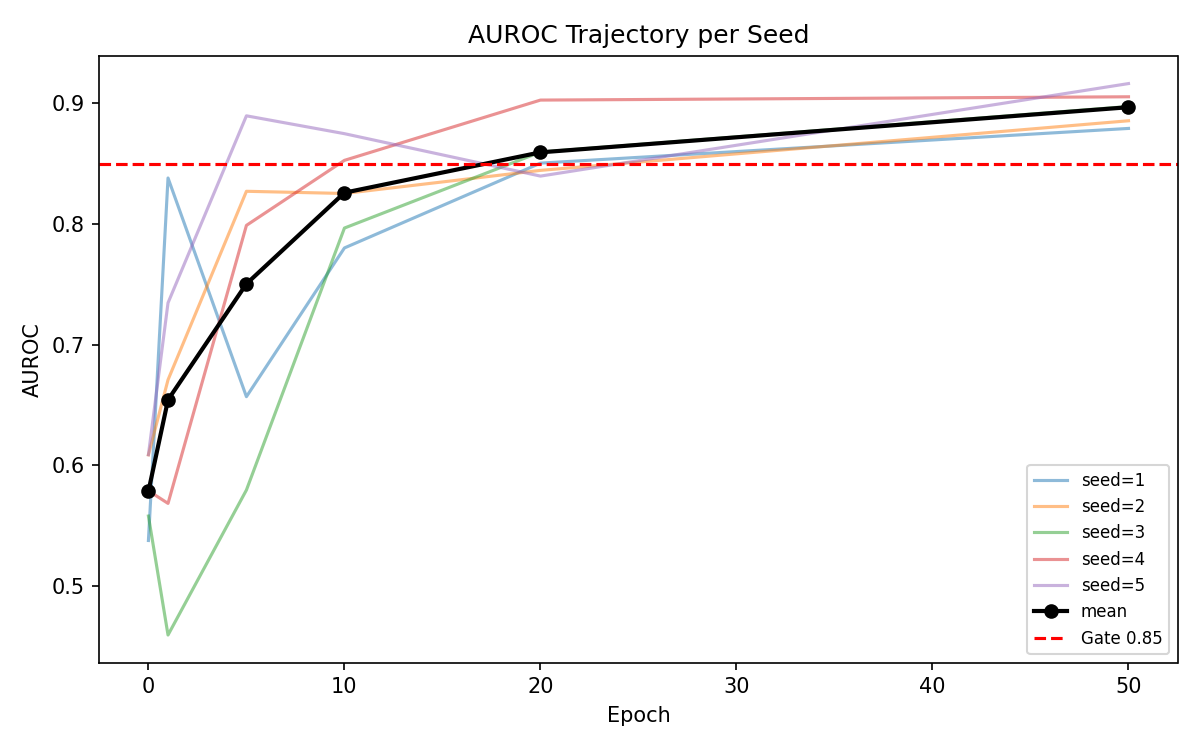
\includegraphics[width=0.8\columnwidth]{figures/fig3_auroc_trajectory.png}
\caption{Full AUROC trajectory across checkpoints $t\in\{0,1,5,10,20,50\}$ for all 5 seeds.}
\label{fig:auroc_trajectory}
\end{figure}

\begin{figure}[h]
\centering
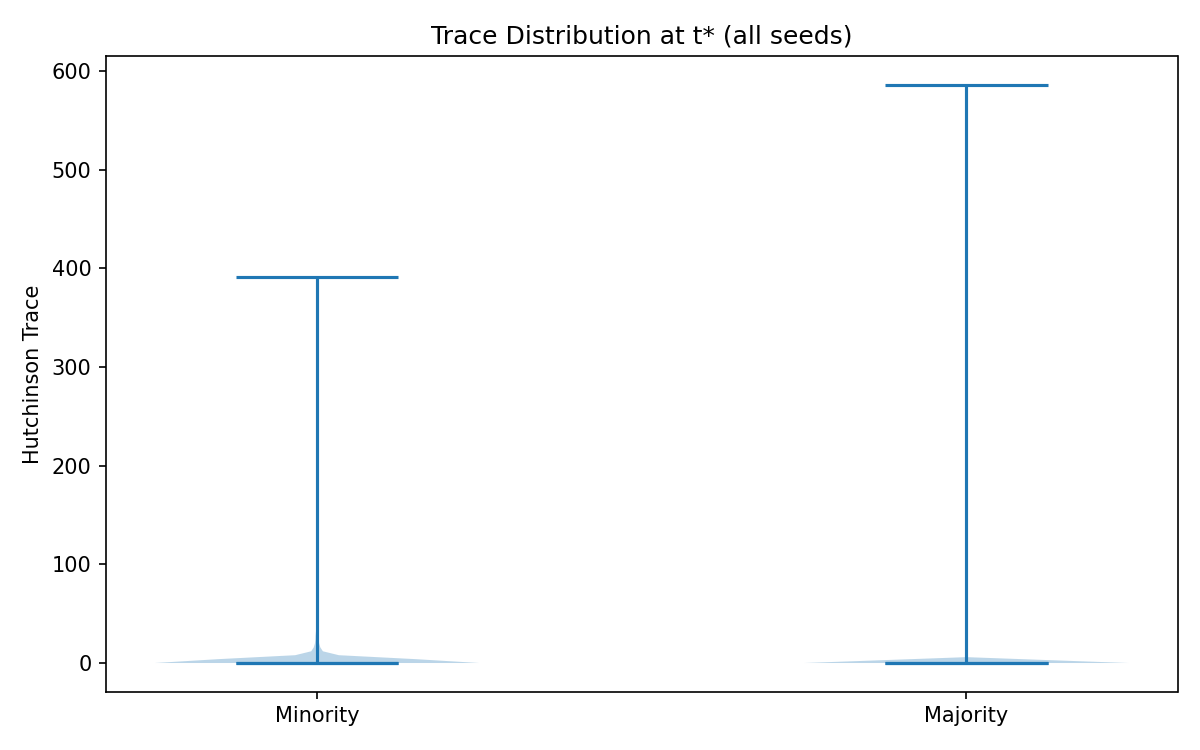
\includegraphics[width=0.8\columnwidth]{figures/fig4_trace_distribution.png}
\caption{Per-sample trace distributions at $t^*$ for minority and majority groups. Minority traces are systematically elevated.}
\label{fig:trace_dist}
\end{figure}

\begin{figure}[h]
\centering
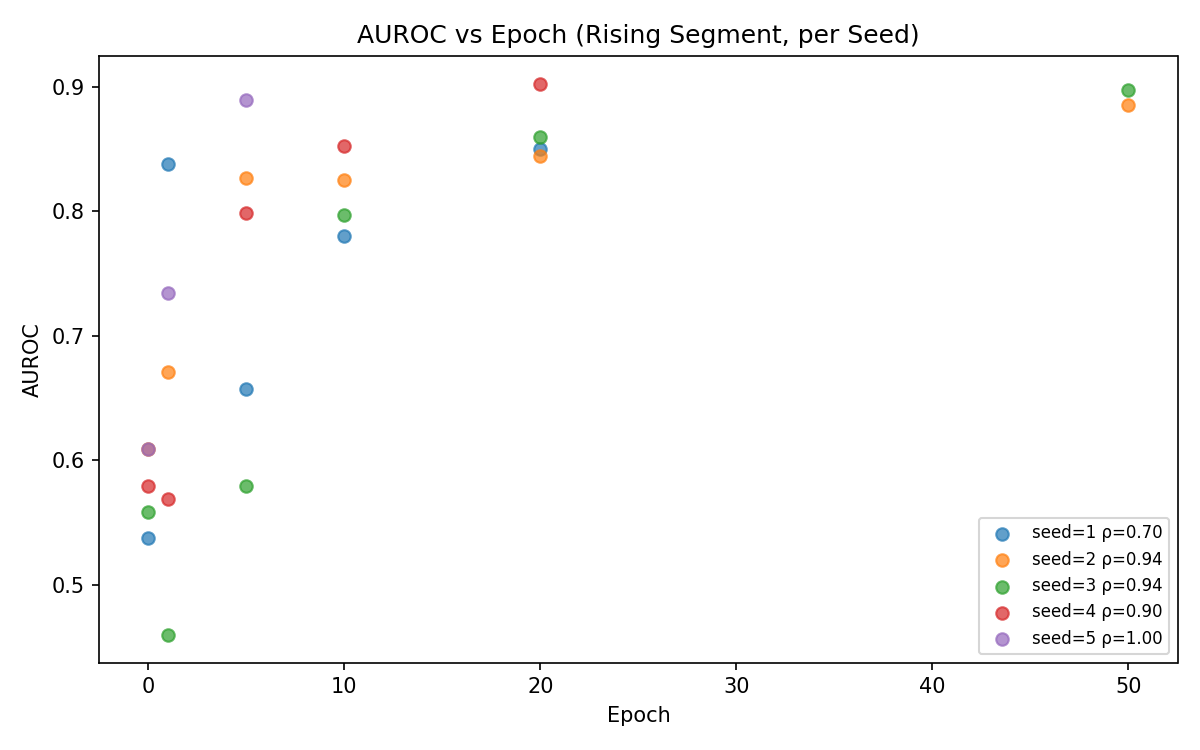
\includegraphics[width=0.8\columnwidth]{figures/fig5_spearman_rising.png}
\caption{Spearman $\rho$ values on the rising AUROC segment per seed.}
\label{fig:spearman}
\end{figure}
